\documentclass[16pt]{article}

\usepackage[english]{babel}
\usepackage[utf8x]{inputenc}
\usepackage{amsmath}
\usepackage{graphicx}
% \usepackage[colorinlistoftodos]{todonotes}
\usepackage[margin=0.8in]{geometry}

\title{AS205:Ocean Dynamics(Assignment 1)}
\author{Parag Shende}

\begin{document}
\maketitle
\hrule

\section{Bathymetry of North Indian Ocean}

We describe the bathymetric features of the North Indian Ocean specifically 
the Arabian Sea and the Bay of Bengal. We use the ETOPO dataset.

\section{North Indian Ocean}

\subsection{Arabian Sea}

\begin{center}
    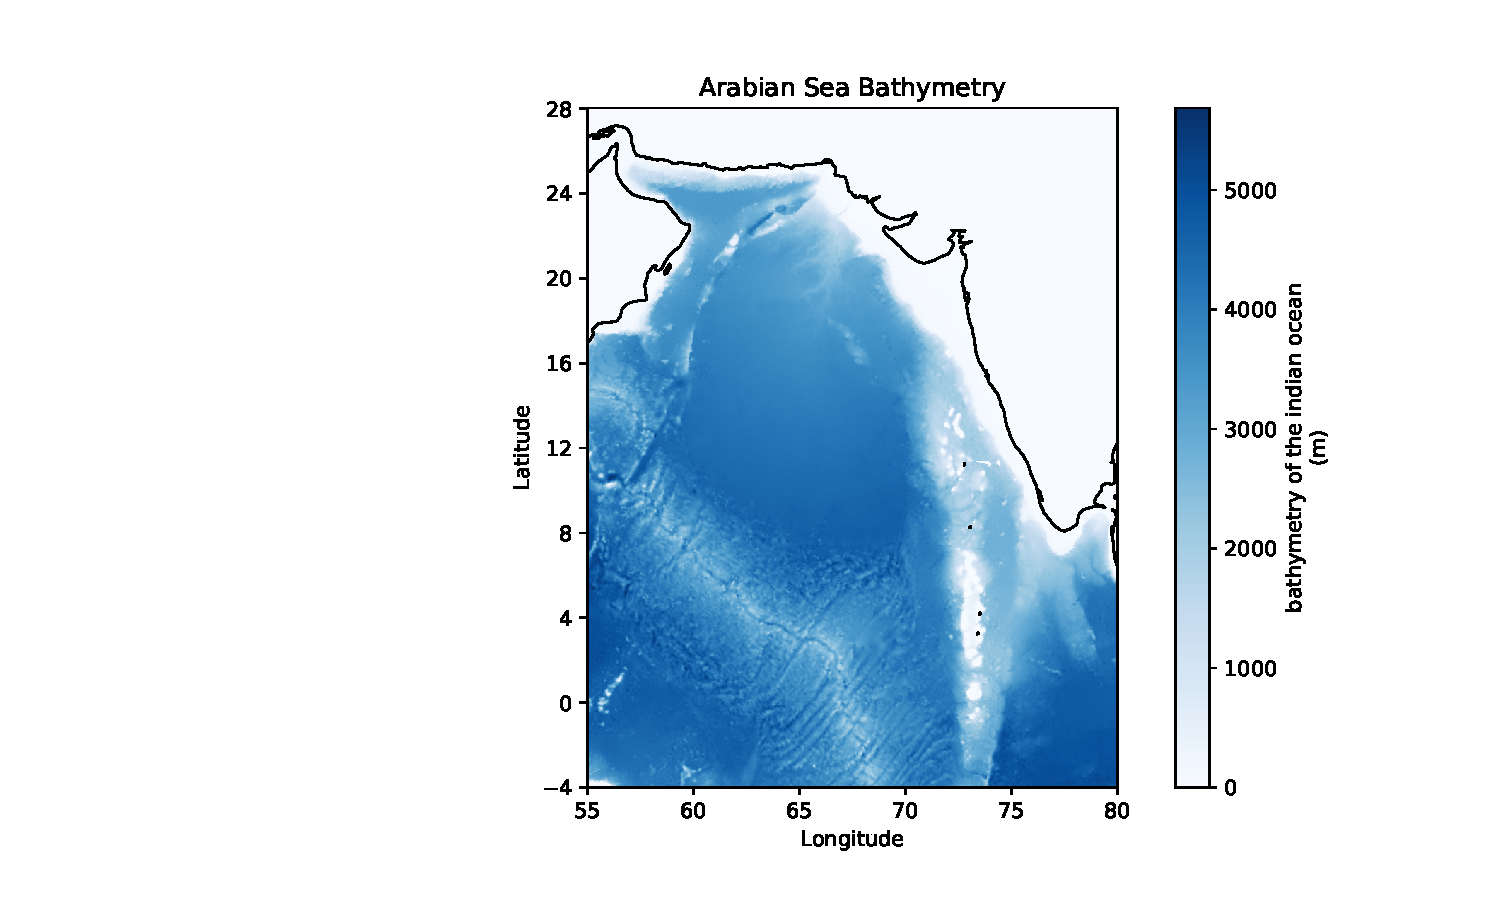
\includegraphics[width=1.0\textwidth]{Arabian_Sea_Bathymetry.png}
\end{center}

\begin{itemize}
\item The Arabian Sea is the western marginal sea of the North Indian Ocean.
\item It is enclosed by the Indian subcontinent in the east and Africa in the west. 
\item The Gulf of Eden and Gulf of Suez are located to the west of Arabian Sea.
\item The Mid-ocean ridge runs in the North-West to South-East direction in the middle of the Arabian Sea.
\item The continental shelf of Indian subcontinent is a prominent feature in the east.
\item The Lakshadweep island shelf is also prominent, located South-West of India. It is also a part of the Chagos-Laccadive ridge.
\end{itemize}

\subsection{Bay of Bengal}

\begin{center}
    \includegraphics[width=1.0\textwidth]{Bay_of_Bengal_Bathymetry.png}    
\end{center}

\begin{itemize}
    \item The Bay of Bengal is the eastern marginal sea of the North Indian Ocean.
    \item It is enclosed by India to the west and the Indochinese peninsula.
    \item It is connected to the Pacific Ocean to the east by Strait of Malaga near the Andaman Sea.
    \item The eastern side has more prominent continental shelf than the western side.
    \item The interior of the Bay of Bengal has nearly uniform abyssal depth of roughly around 4000-5000m.
    \item The ninety-east ridge is located in the southern Bay of Bengal around 89.0 E longitude and reaching upto 4 N latitude.
\end{itemize}

\end{document}